\section{Evaluation}
\label{sec:evaluation}

We now evaluate the data transfer overhead in the context of cloud-based
autonomous driving.
We assume that autonomic control and environmental perception are
provided in the remote server, but they are not within the scope of this
paper.
What we focus on in this experiment is the measurement of the data
transfer overhead.
Throughout the experiment, we assume that WiFi (IEEE802.11n
2.4GHz/5.0GHz) is provided with bandwidth of 300Mbps while LTE (au
2.1GHz LTE) achieves 75Mbps for downstream and 25Mbps for upstream.


\subsection{Control Command Transfer}

This experiment measures the transfer time taken to send control
commands to the vehicle from a smartphone.
The commands control the steering, accel, and brake of the vehicle.
The steering angle is determined by the gyro sensor data while the accel
and break strokes are manipulated by the graphics user interface of the
Andrive application.
We use the HTC J butterfly Snapdragon S4 Pro (APQ8064@1.5GHz, Quad Core)
for a testing smartphone.

\begin{figure}[!t]
 \centering
 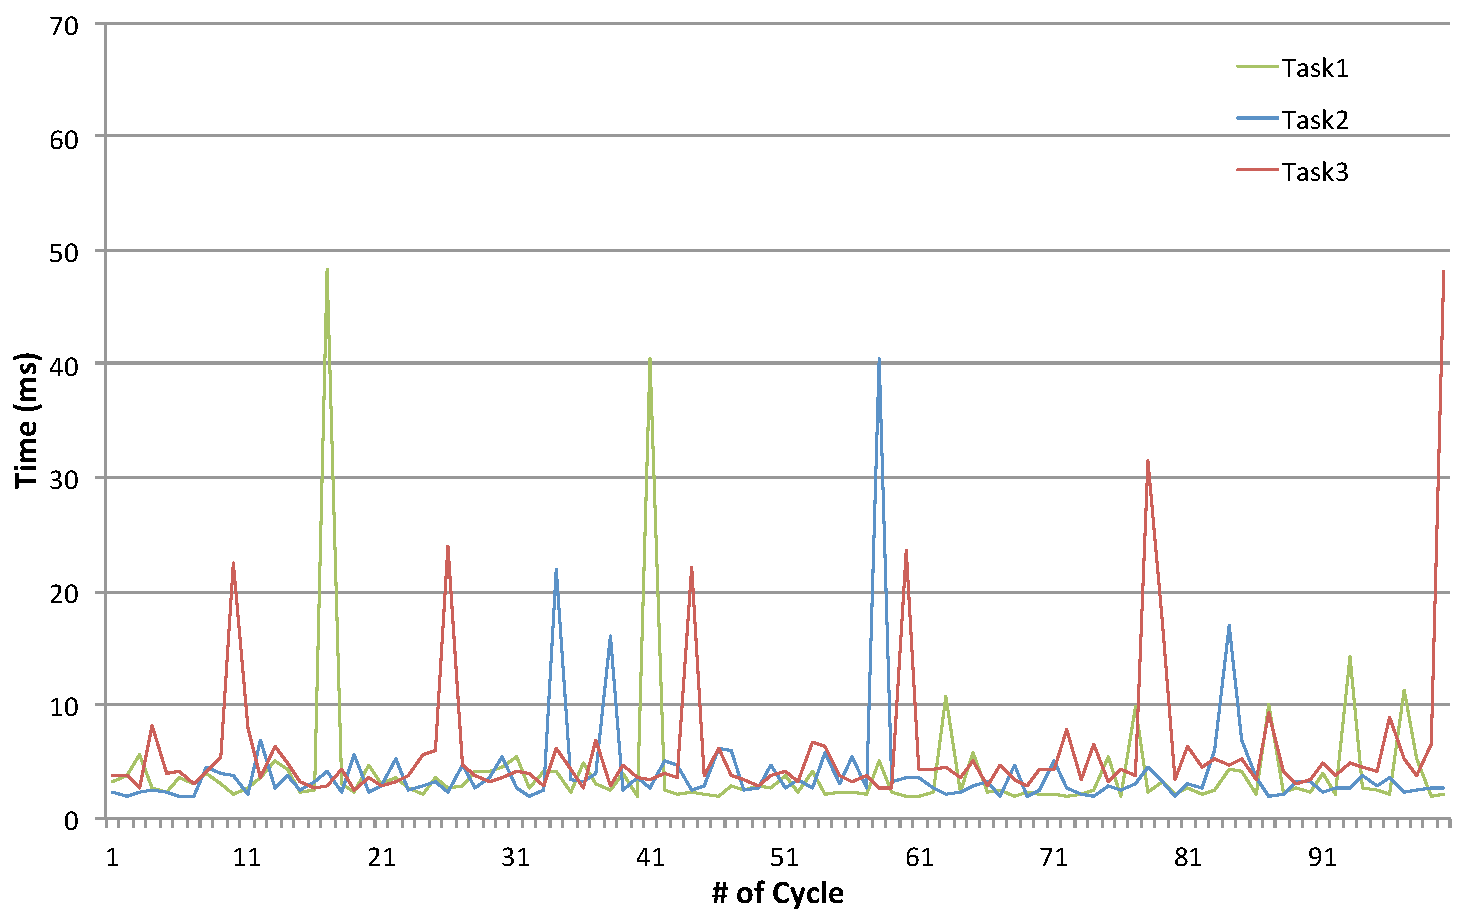
\includegraphics[width=0.8\hsize]{fig/No1_Andrive_serv_cycle_WiFi.pdf}
 \caption{The achieved period of \textit{synchronous} data transfers for
 control commands using WiFi.}
 \label{fig:no1}
 \vspace{1em}
 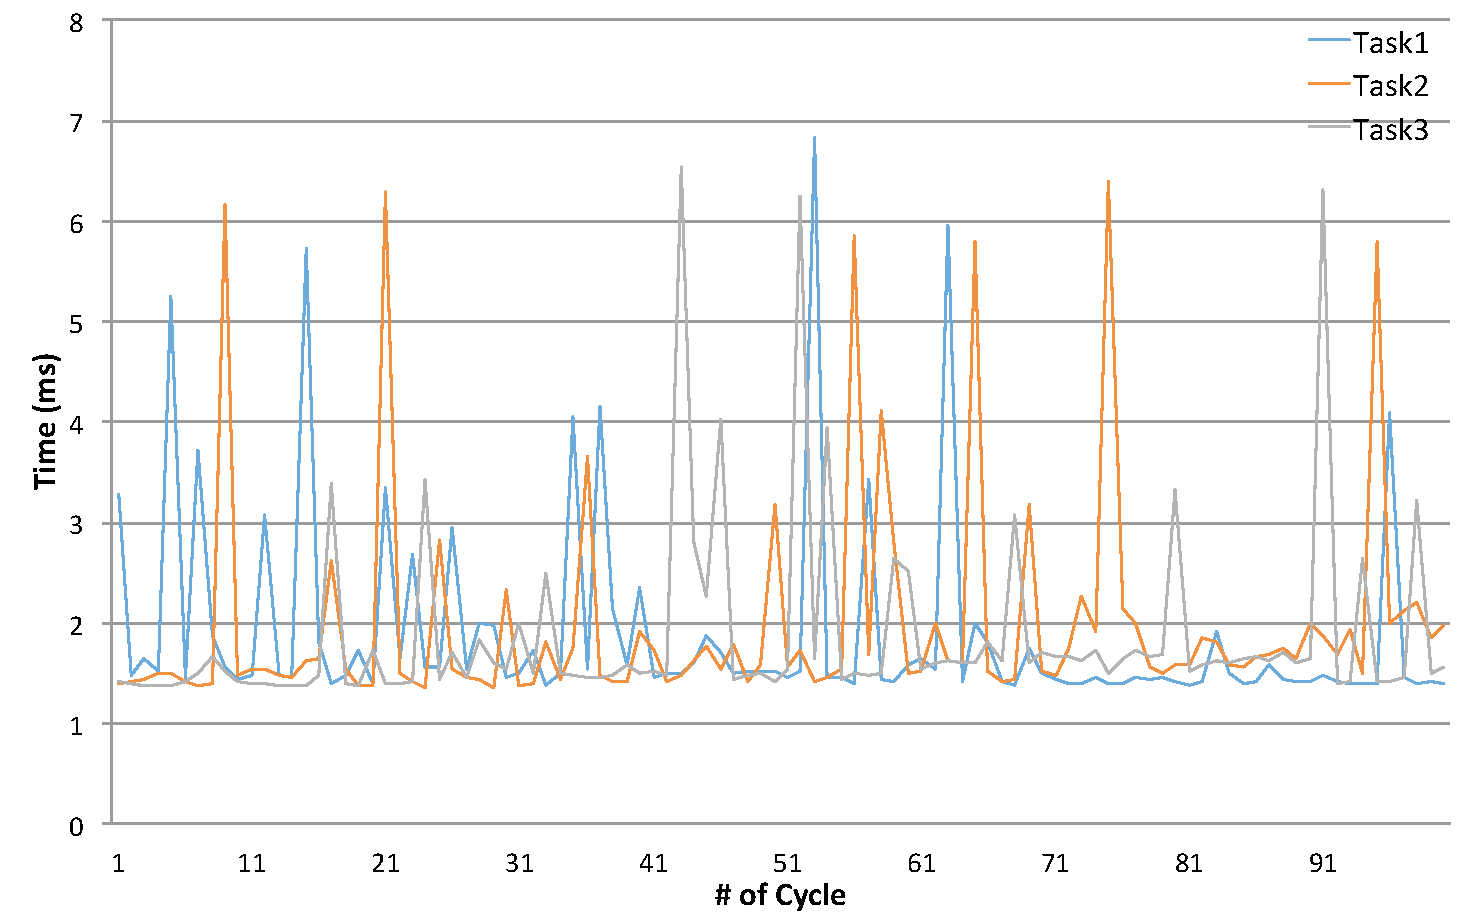
\includegraphics[width=0.8\hsize]{fig/No4_Andrive_serv_cycle_WiFi_only_send.pdf}
 \caption{The achieved period of \textit{asynchronous} data transfers
 for control commands using WiFi.}
 \label{fig:no4}
\end{figure}

Fig. \ref{fig:no1} shows the period (interarrival time) of data
transfers for vehicle control commands achieved using WiFi when the
vehicular master computer in the vehicle and a client smartphone are
synchronized.
The nodes are connected within a local area network, and the vehicular
master computer sends back an acknowledgement message to the smartphone
every time the commands are received for synchronization.
It meets a period of $5ms$ on average, which is acceptable for the
feedback control rate of autonomous driving \cite{Kagami13}.
However there are unpredictable spikes that increase the period up to
$60ms$ in the worst case.
These unpredictable spikes are not acceptable under real-time
constraints.

Fig. \ref{fig:no4} shows the period of data transfers in the same
setup as Fig. \ref{fig:no1} except that the vehicular master computer and
the smartphone are not synchronized, \textit{i.e.}, the smartphone is
sending data without waiting for the acknowledgement message from the
vehicular master computer.
It is clear that some spikes are removed as compared to
Fig. \ref{fig:no1}.

\begin{figure}[!t]
 \centering
 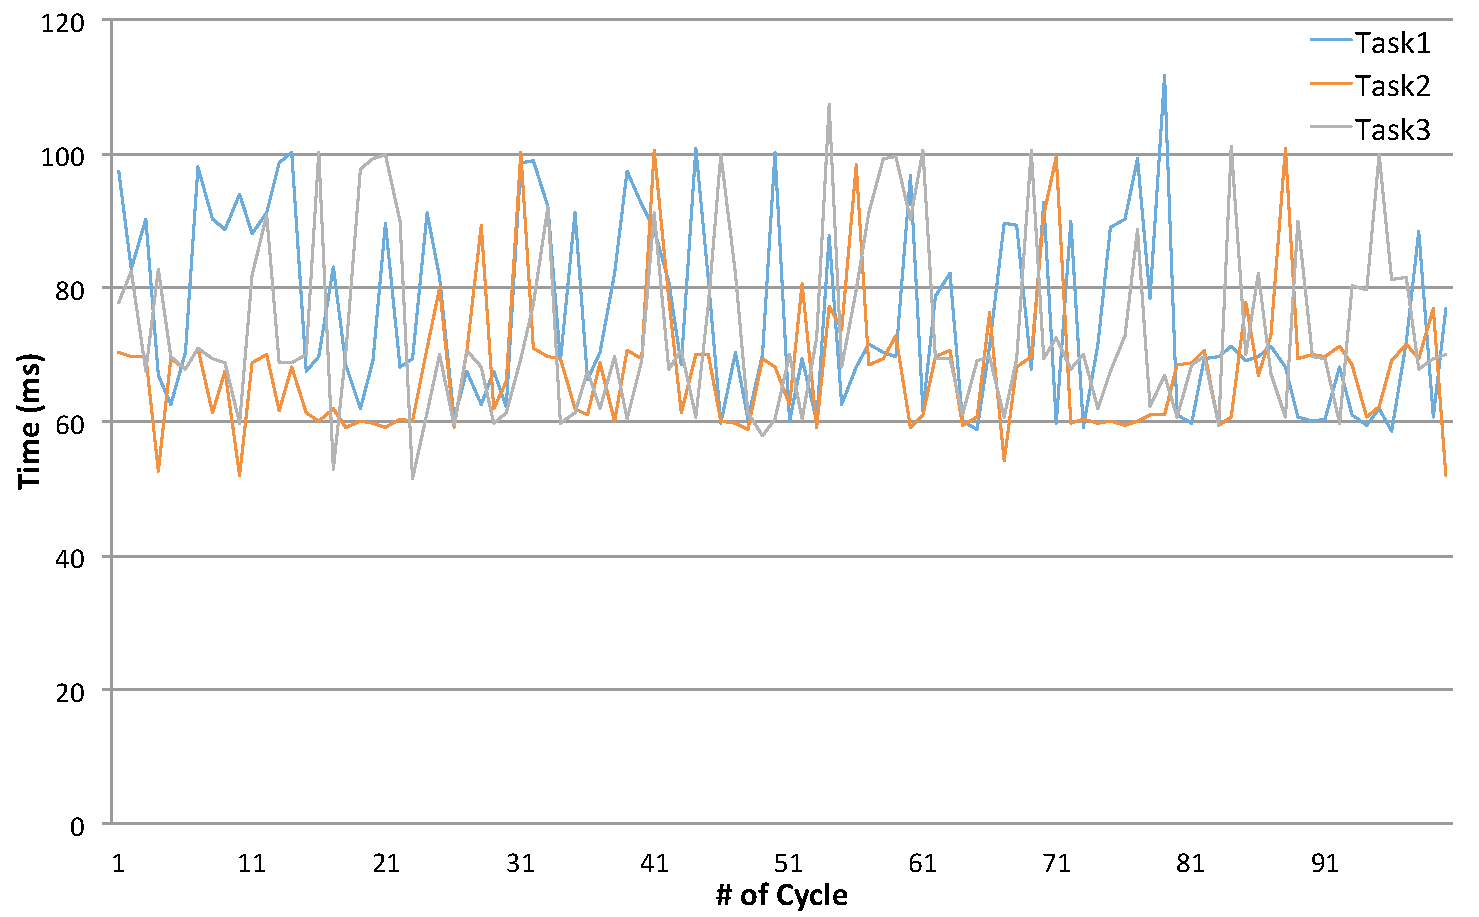
\includegraphics[width=0.8\hsize]{fig/No2_Andrive_serv_cycle_LTE.pdf}
 \caption{The achieved period of \textit{synchronous} data transfers for
 control commands using LTE.}
 \label{fig:no2}
 \vspace{1em}
 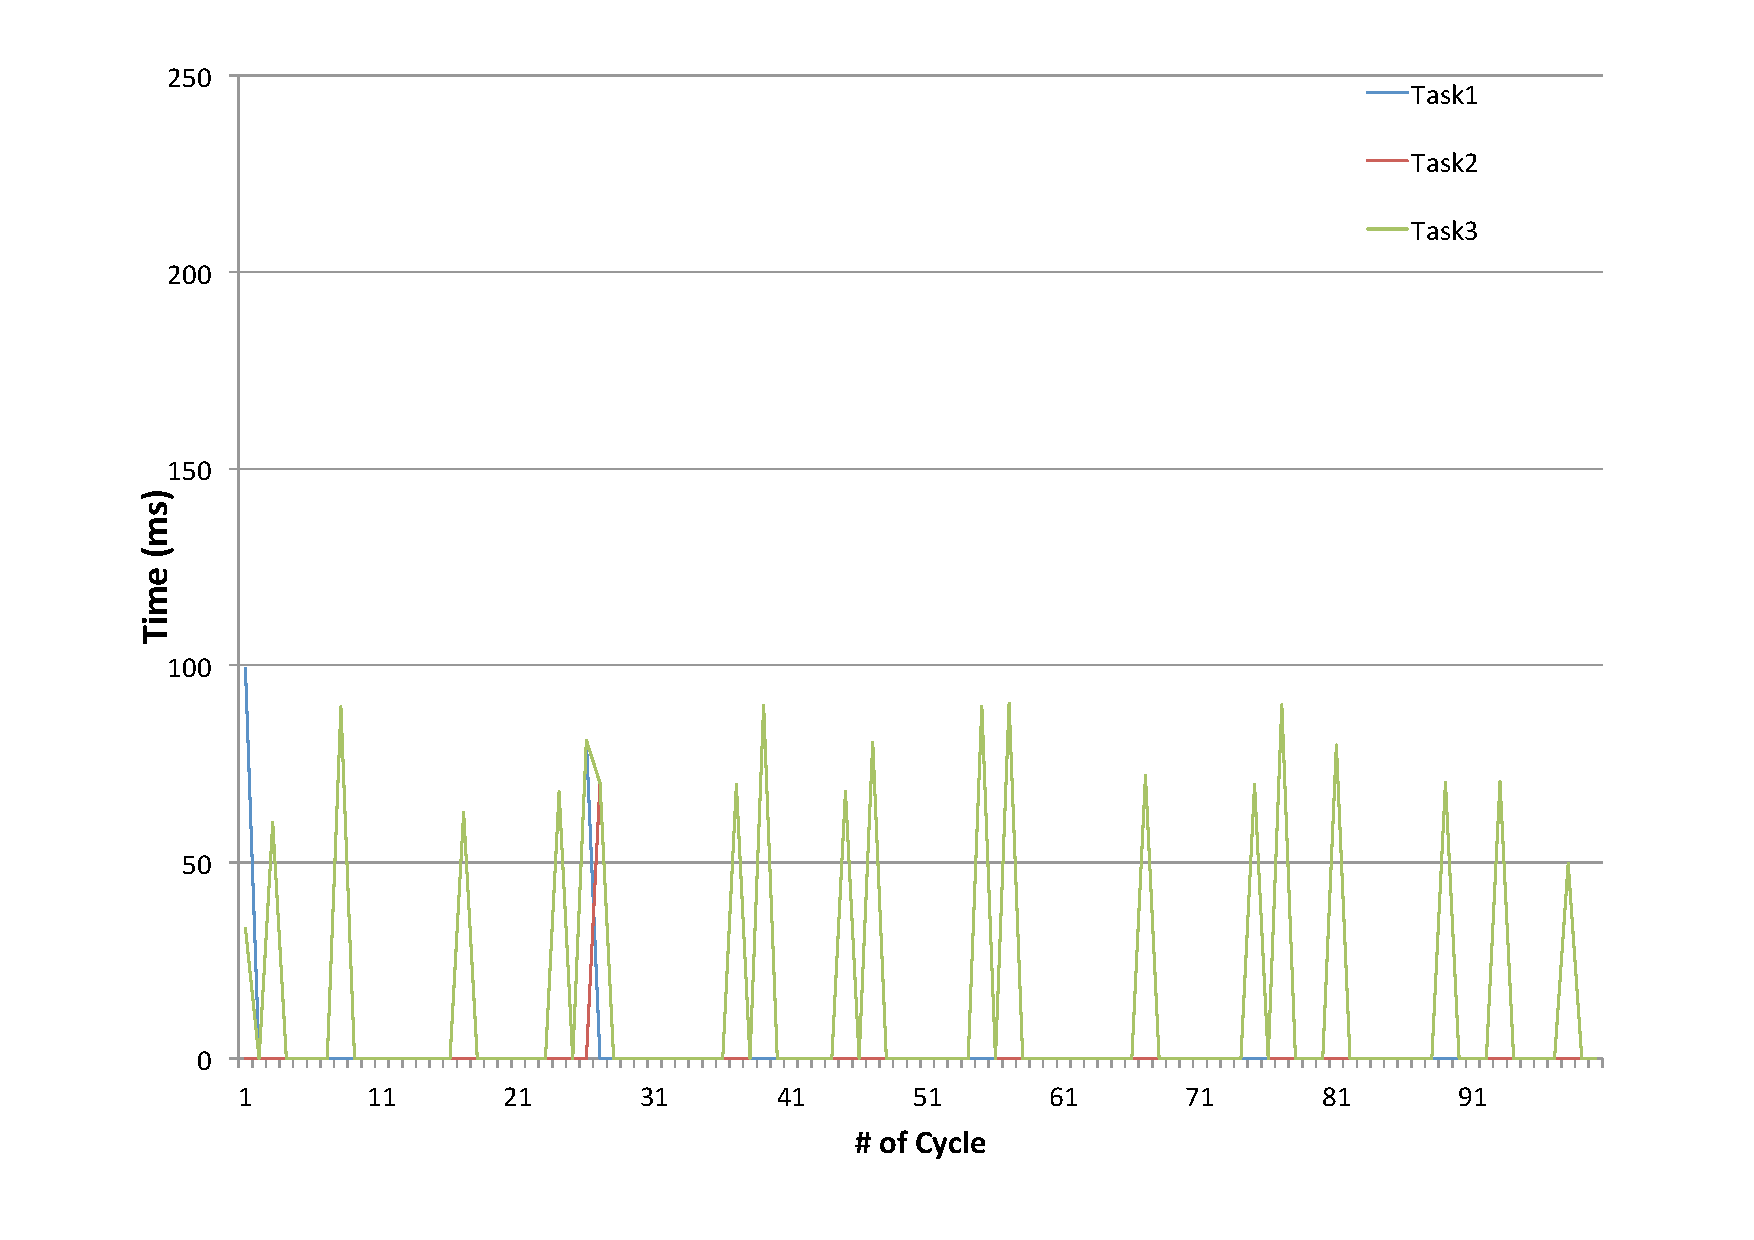
\includegraphics[width=0.8\hsize]{fig/No5_Andrive_serv_cycle_LTE_only_send.pdf}
 \caption{The achieved period of \textit{asynchronous} data transfers for
 control commands using LTE.}
 \label{fig:no5}
\end{figure}

Fig. \ref{fig:no2} and \ref{fig:no5} show the period of data transfers
for the same vehicular control command set using LTE.
While WiFi is often suitable for intranet usage, LTE is more publicly
deployed in the city as part of wireless internet services.
As compared to WiFi, the data transfer times are increased due to less
bandwidth.
Its device specification and device driver implementation are also
different from those of WiFi.
For example, the LTE device driver on the Android smartphone buffers
some data and then transfers a bundle of them at some point.
This characteristics of LTE lead to the zig zag periods of data
transfers as shown in Fig. \ref{fig:no5}.
It is also remarkable that LTE severely suffers from the latency posed
due to waiting for acknowledgement messages.
When using LTE to send data from the global server to the smartphone, a
public base station must detect the location of the smartphone first and
next deliver data.
We suspect that the significant latency comes from this public behavior
of LTE.

\begin{figure}[!t]
 \centering
 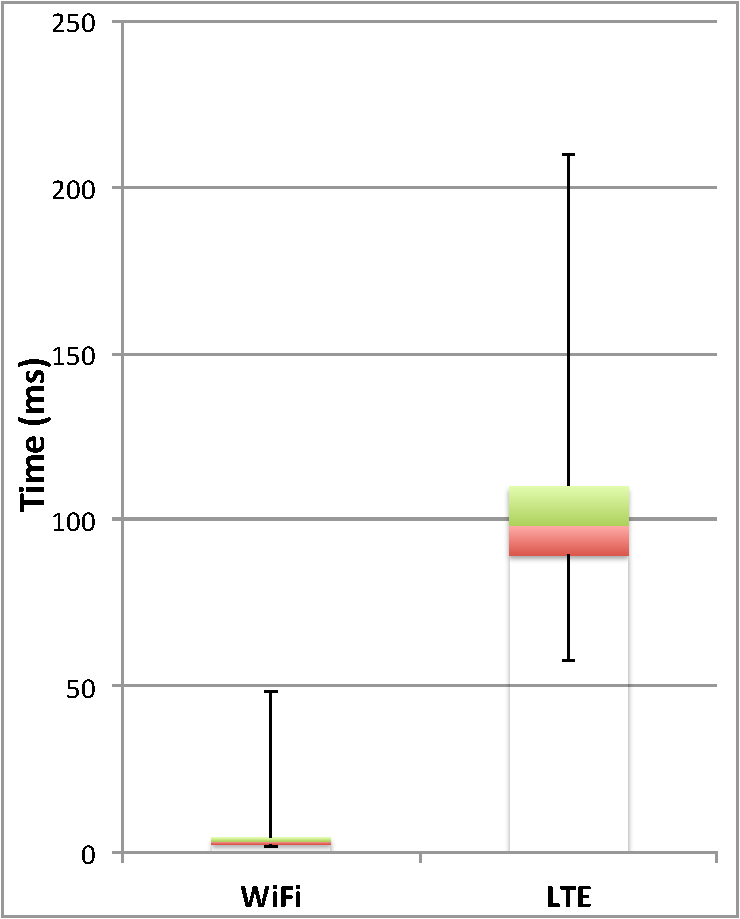
\includegraphics[width=0.45\hsize]{fig/No3_Andrive_boxplot_compare_WiFi_and_LTE.pdf}
 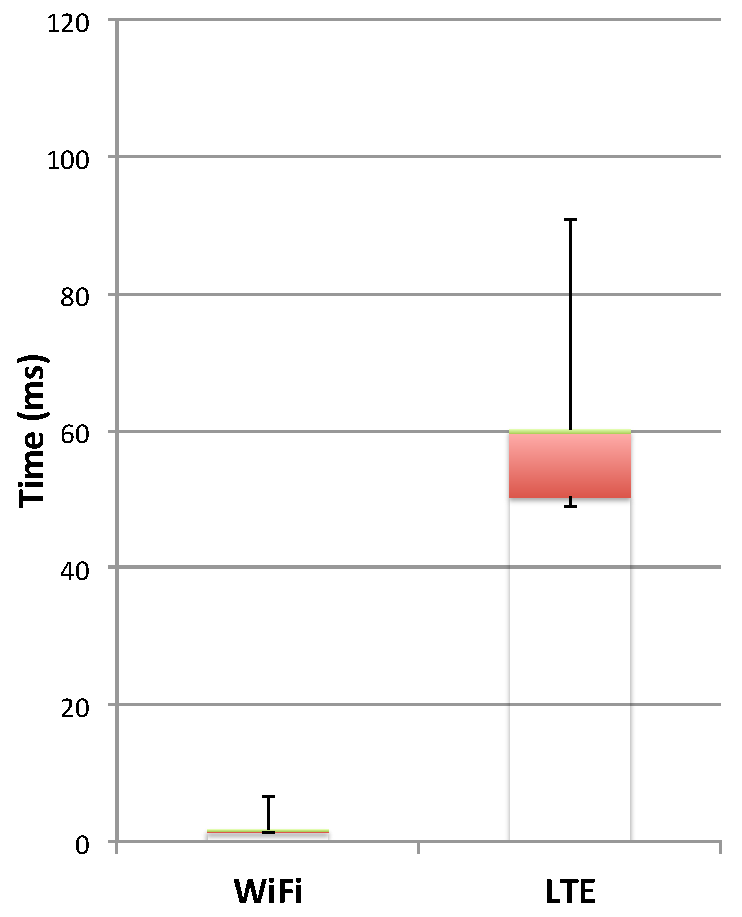
\includegraphics[width=0.45\hsize]{fig/No7_Andrive_only_send_boxplot_compare_WiFi_and_LTE.pdf}
 \caption{Summarized box plotting of the \textit{synchronous} (left) and
 \textit{asynchronous} (right) transfer times.}
 \label{fig:no3_7}
\end{figure}

Fig. \ref{fig:no3_7} depicts summarized box plotting of the achieved
data transfer periods for vehicular control commands.
This explains that WiFi is currently a better choice for real-time
communication using commodity ICT platforms.
We hope that LTE will become more practical for real-time usage given
that it is a publicly available network.

\subsection{Image Transfer}

\begin{figure}[!t]
 \centering
 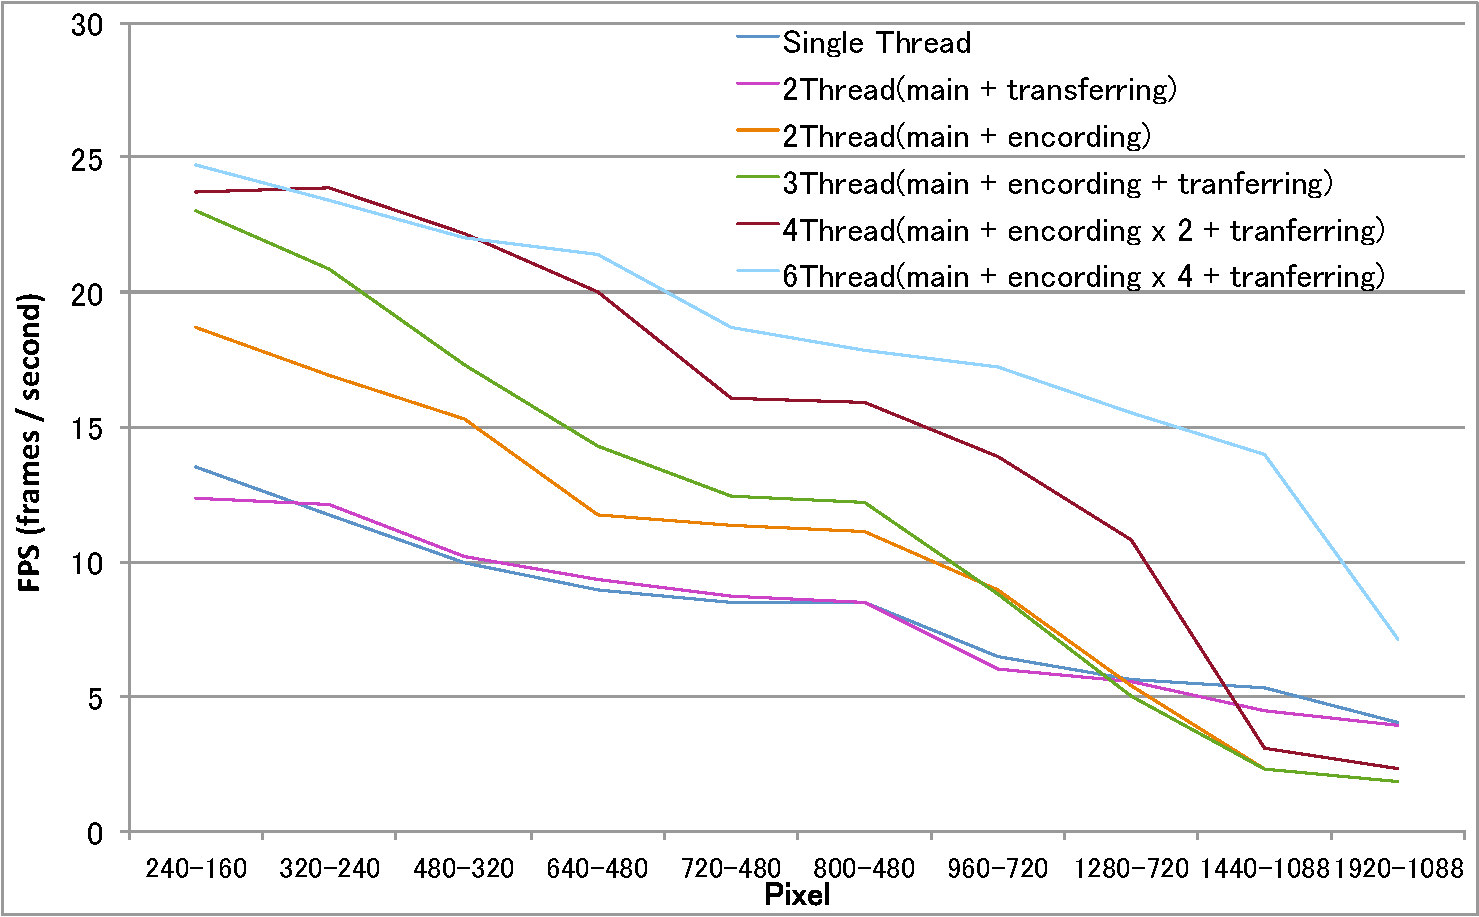
\includegraphics[width=0.8\hsize]{fig/No8_TIPiC_FPS_graph_WiFi.pdf}
 \caption{The frame rate of image transfers using WiFi.}
 \label{fig:no8}
\end{figure}

Fig. \ref{fig:no8} shows the average frame rate of image transfers
achieved using WiFi.
We provide six variants of the image transfer program running on the
smartphone.
As described in Section \ref{sec:prototype}, the throughput of image
transfers can be improved by multithreading.
The top label (Single Thread) uses only a single thread to capture,
encode, and transfer images.
The other labels represent such implementations that use pipelining with
multithreading.
Espeically the stage of encoding is time consuming, we also use multiple
threads for encoding itself.
It is notable that using four or six threads in total, we can meet a
frame rate of more than $20$fps for a standard image size of $640 \times
480$ pixels.
This is a useful finding that we could use smartphones with WiFi to
offload image processing to the cloud in terms of frame rate.

\begin{figure}[!t]
 \centering
 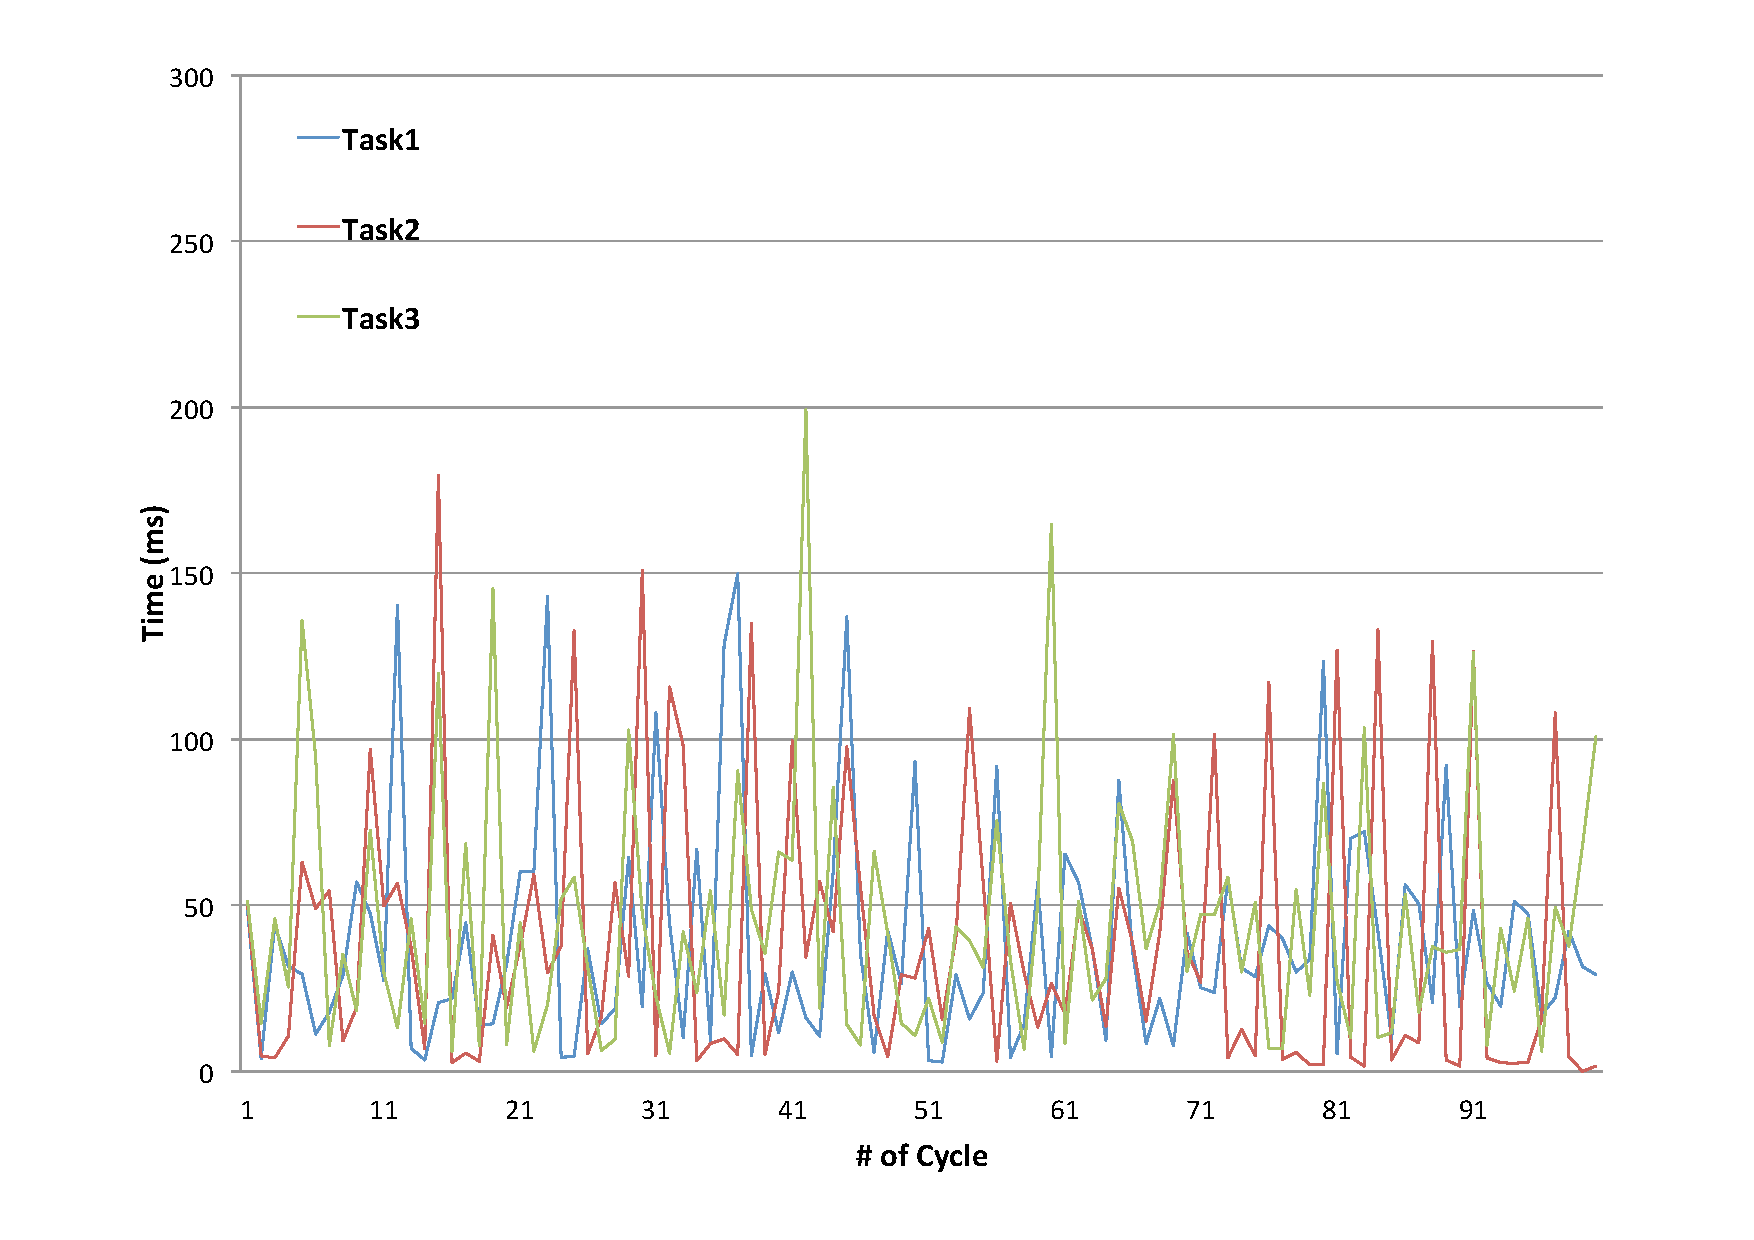
\includegraphics[width=0.8\hsize]{fig/No9_TIPiC_serv_cycle_WiFi.pdf}
 \caption{The achieved period of image transfers using WiFi.}
 \label{fig:no9}
\end{figure}

Fig. \ref{fig:no9} shows the period of image transfers on a cycle bais
achieved using WiFi.
Albeit high frame rates demonstrated in Fig \ref{fig:no8}, the period is
actually fluctuating to an extent.
For example, some spike reaches $200ms$.
This unpredicted spike may jeopardize fine-grained control that actuates
based on the results of image processing but it also depends on the
algorithm.
From this experiment, therefore, we conclude that the algorithm of
control using the results of networked image processing must be designed
to be dependable against timing jitters.

\begin{figure}[!t]
 \centering
 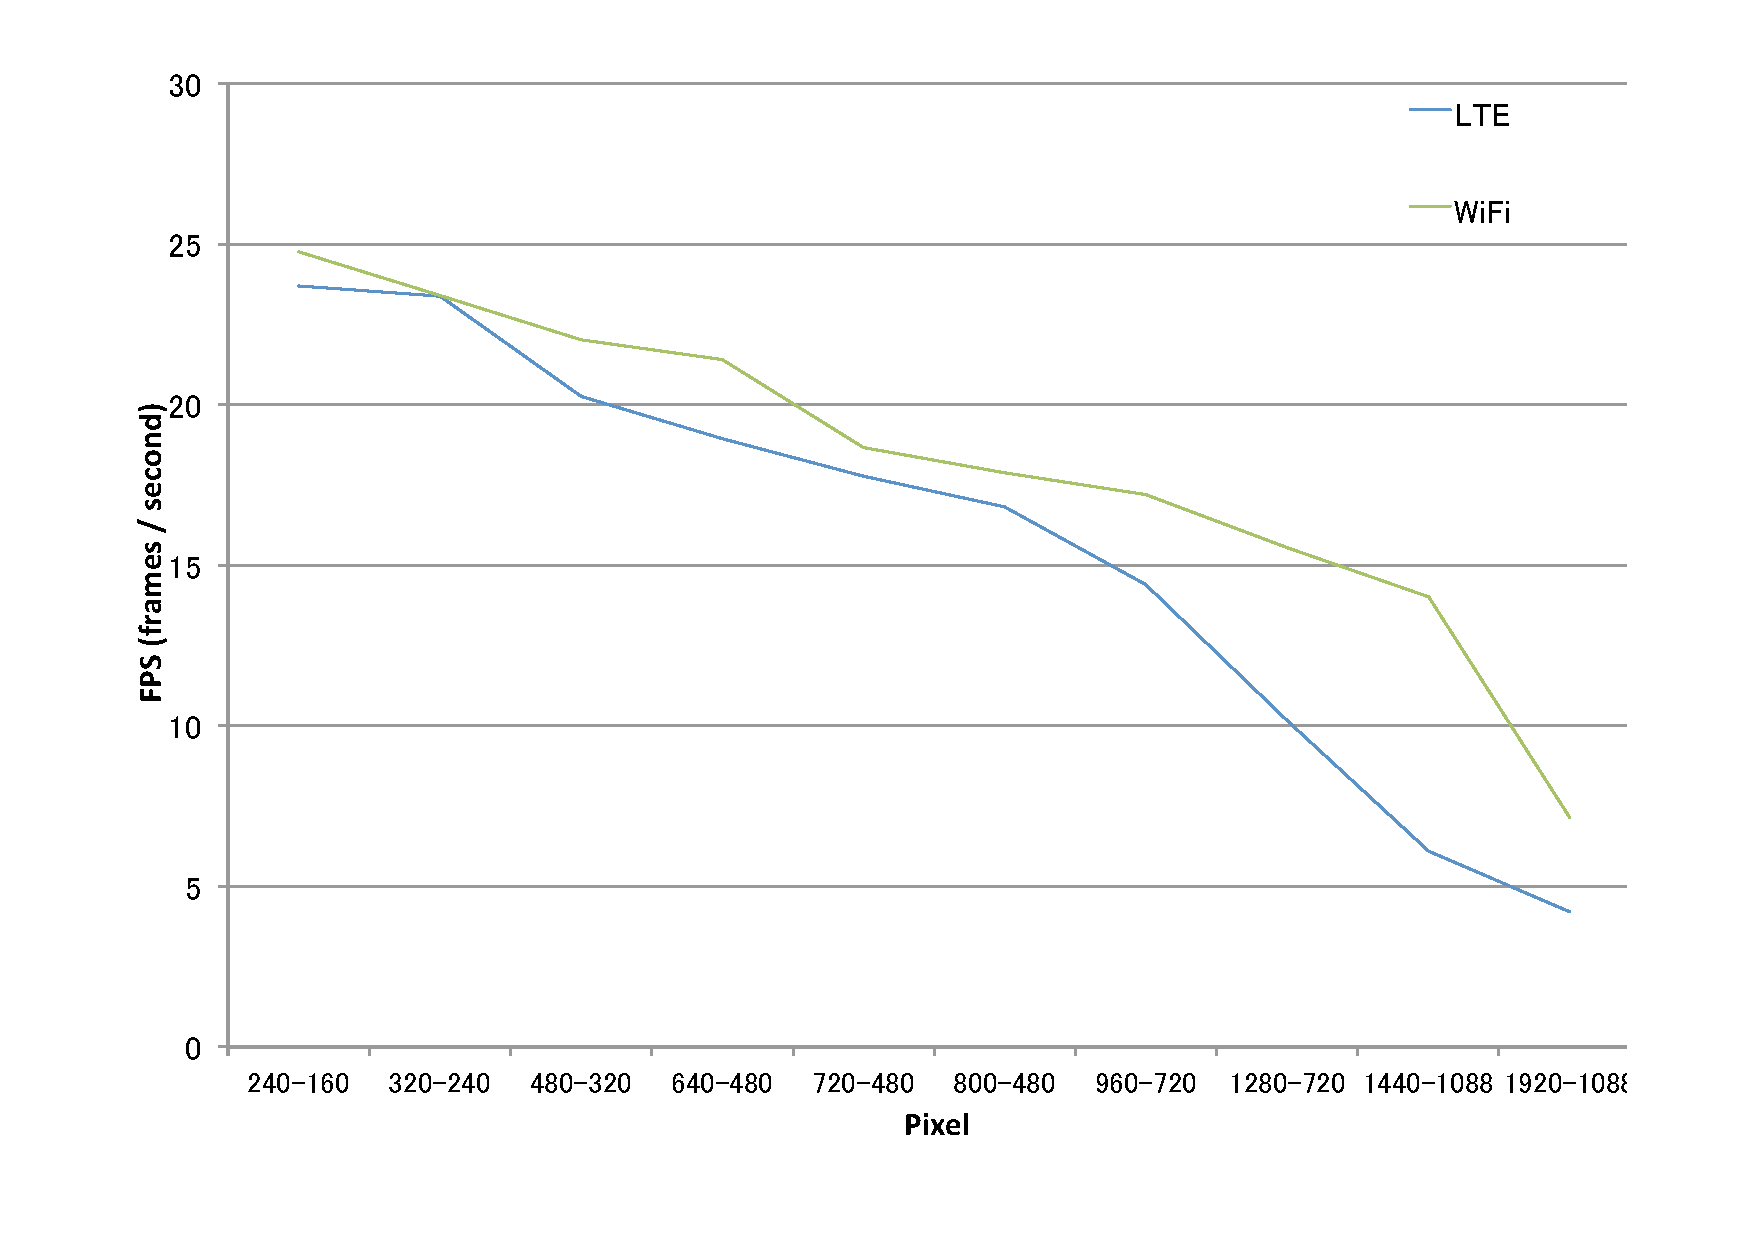
\includegraphics[width=0.8\hsize]{fig/No10_TIPiC_FPS_graph_LTE.pdf}
 \caption{The frame rate of image transfers using LTE.}
 \label{fig:no10}
\end{figure}

\begin{figure}[!t]
 \centering
 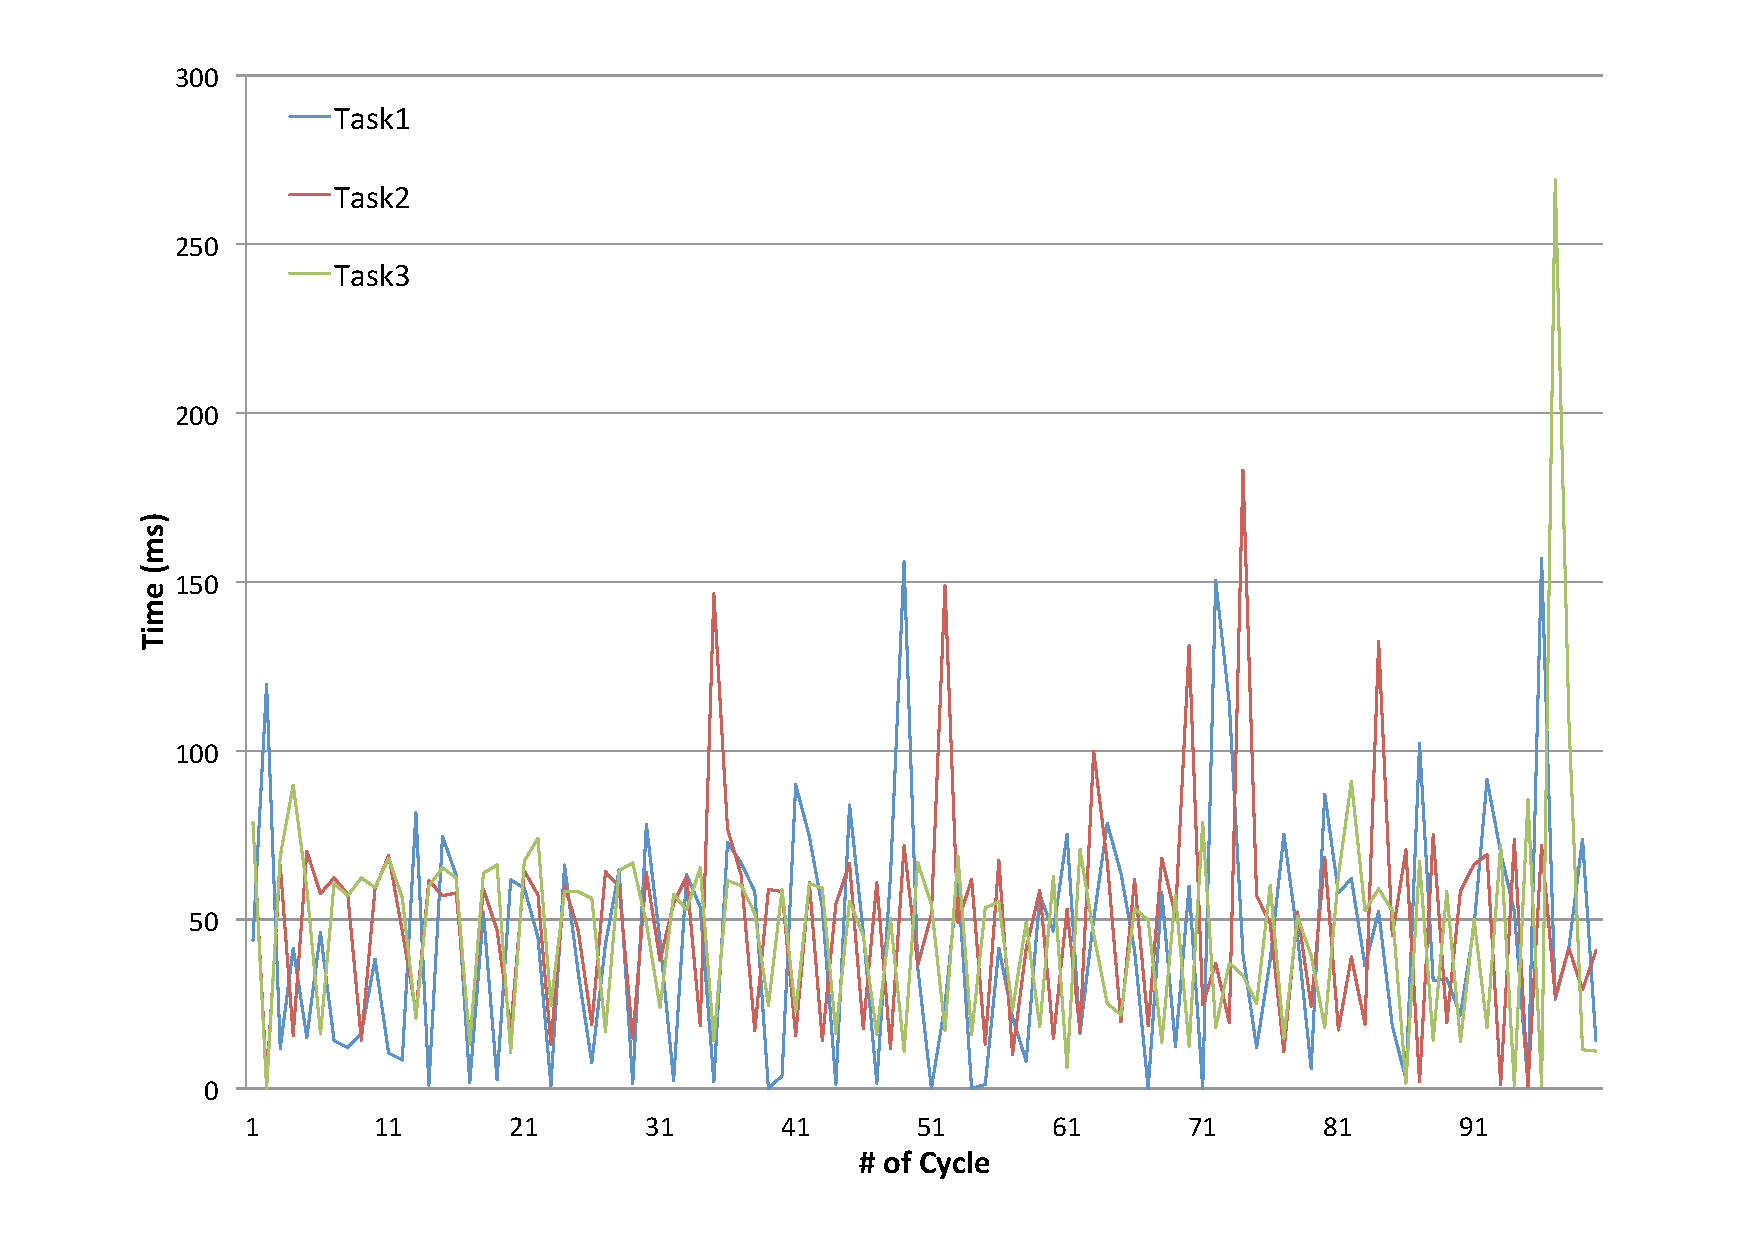
\includegraphics[width=0.8\hsize]{fig/No11_TIPiC_serv_cycle_LTE.pdf}
 \caption{The achieved period of image transfers using LTE.}
 \label{fig:no11}
\end{figure}

Fig. \ref{fig:no10} and \ref{fig:no11} show the frame rate and the
period achieved using LTE for the same image transfers as those shown in
Fig. \ref{fig:no8} and \ref{fig:no9}.
Unlike the case of control commands that highlighted the latency, the
frame rate and the period of image transfers are not very different
between WiFi and LTE.
Since we use a smartphone employing an embedded processor, we consider
that throughput is dominated by the processor performance rather than
the network performance.
This means that LTE is competitive to WiFi in throughput as far as we
use a smartphone as a client device.

\begin{comment}
\begin{figure}[!t]
 \centering
 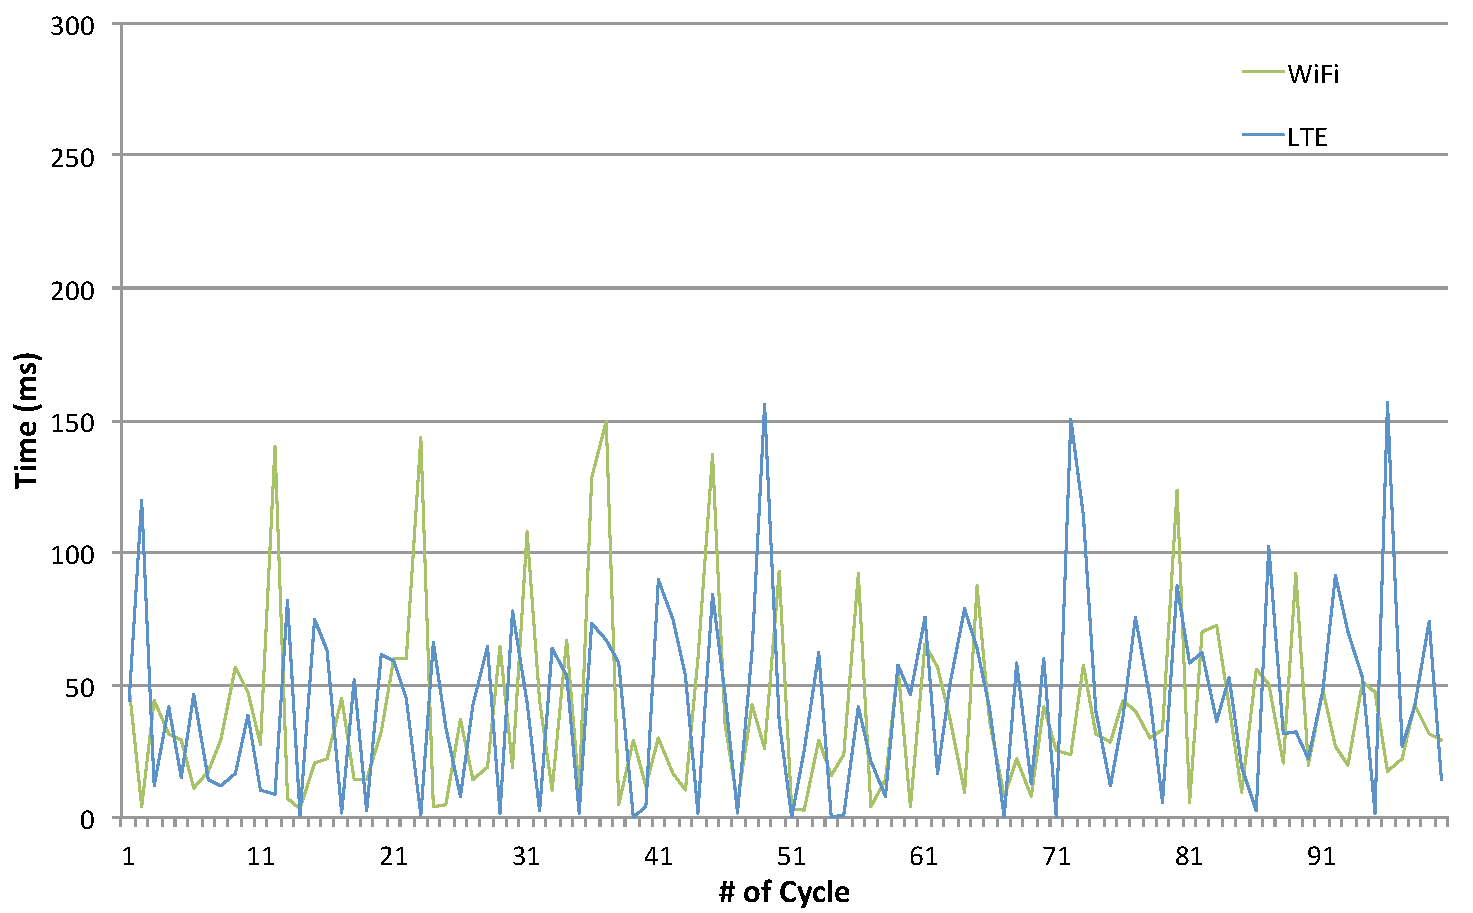
\includegraphics[width=0.8\hsize]{fig/No12_TIPiC_serv_cycle_compare_WiFi_and_LTE.pdf}
 \caption{A comparison of the arrival times.}
 \label{fig:no12}
\end{figure}

\begin{figure}[!t]
 \centering
 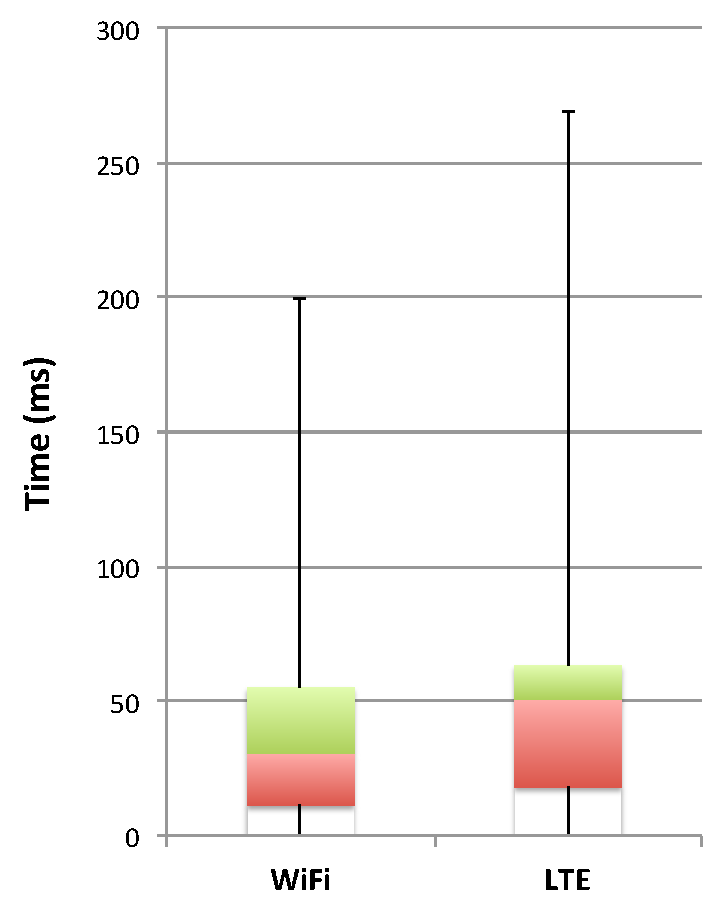
\includegraphics[width=0.5\hsize]{fig/No13_TIPiC_boxplot_compare_WiFi_and_LTE.pdf}
 \caption{Summarized box plotting of the arrival times.}
 \label{fig:no13}
\end{figure}
\end{comment}

\begin{figure}[!t]
 \centering
 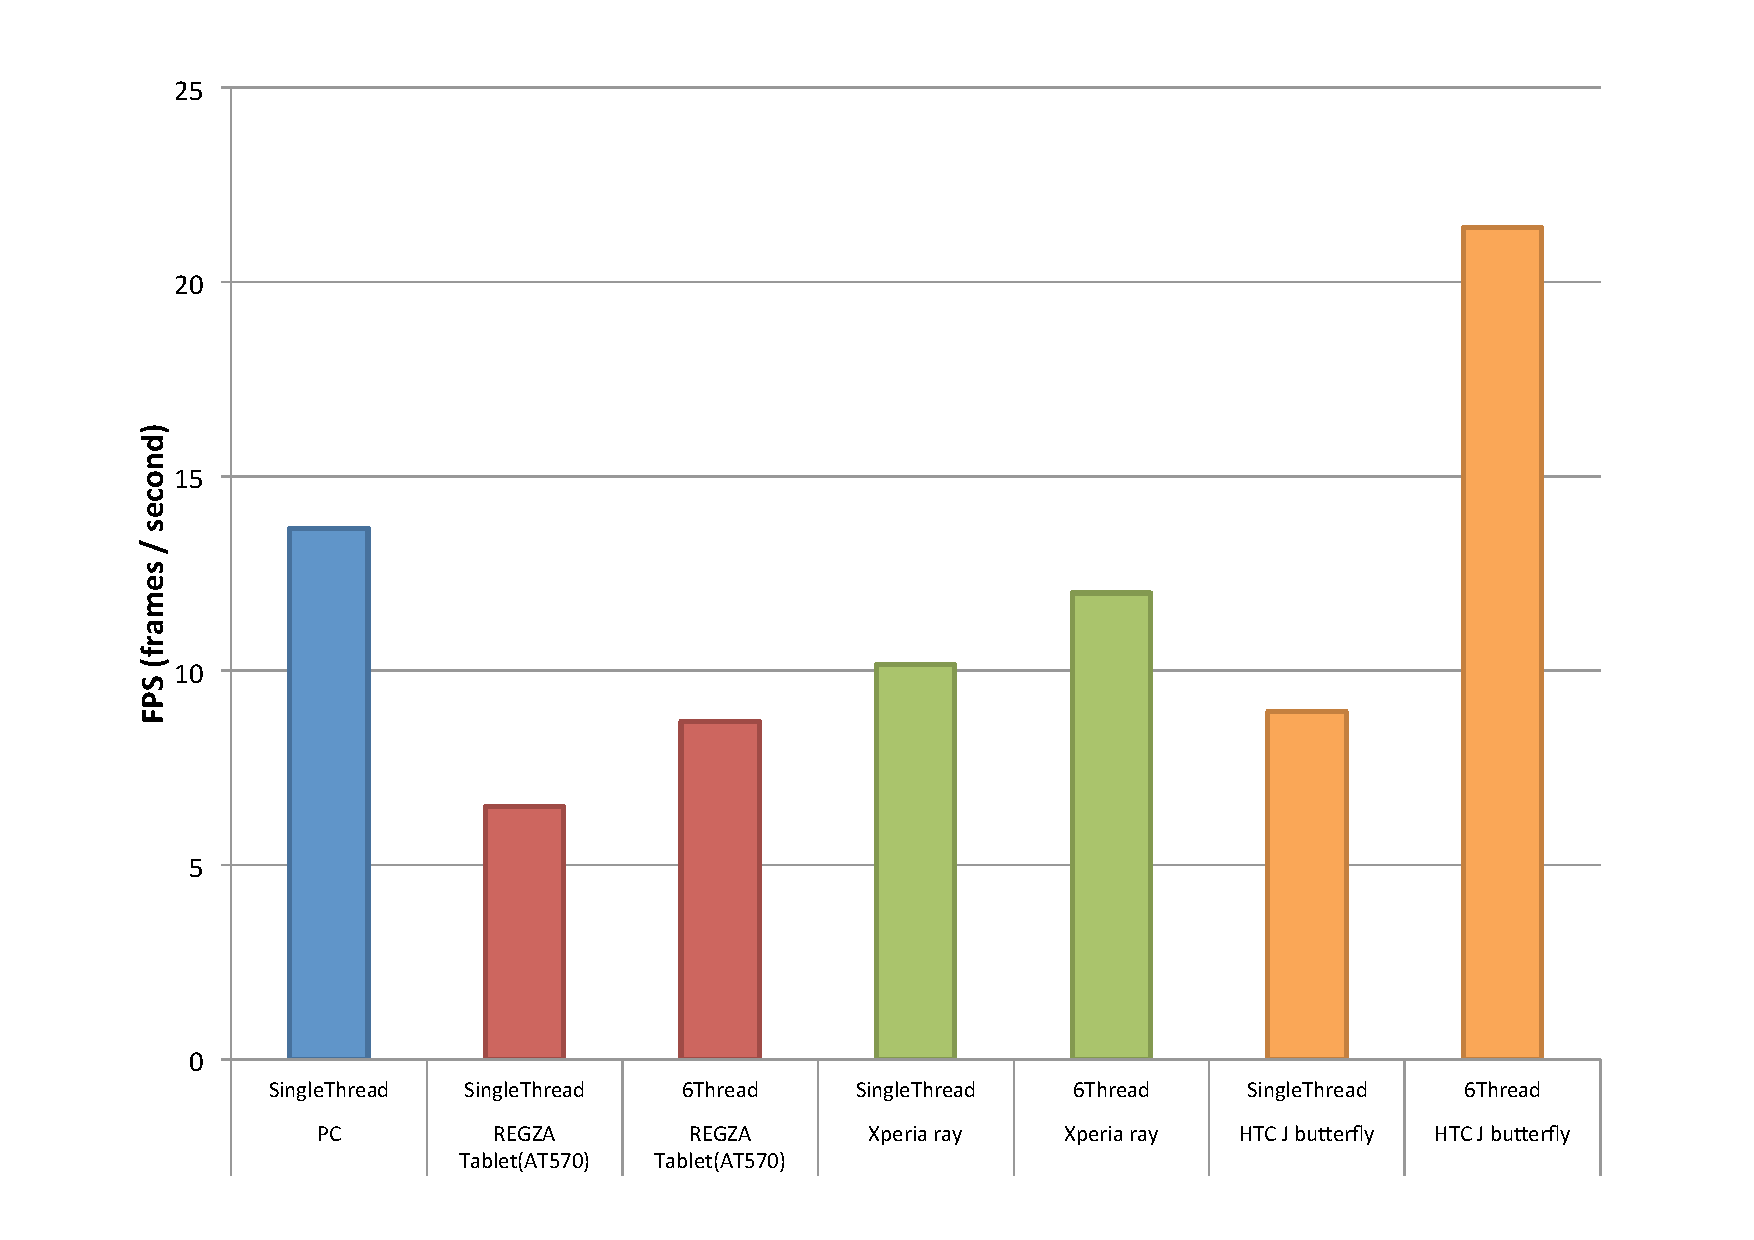
\includegraphics[width=0.8\hsize]{fig/No14_Android_and_PC_benchmarck.pdf}
 \caption{Performance differences among smartphones}
 \label{fig:no14}
\end{figure}

Fig. \ref{fig:no14} shows performance differences among various
smartphones.
For a reference, we also plot the performance of a single threaded PC.
It shows that the performances of smartphones are getting very powerful
especially when multithreading is activated.